\section{仿射簇的乘积}\label{sec:products-of-affine-varieties}

给定仿射簇 $X\subseteq\mathbb{A}^{m}$ 和 $Y\subseteq\mathbb{A}^{n}$, 从集合论角度, 它们的 Cartesian 积 $X\times Y$ 就是下列有序对的集合:
\[
  X\times Y=\{(a,b)\mid a\in X,\ b\in Y\}\subseteq\mathbb{A}^{m}\times\mathbb{A}^{n}.
\]
\BookPairedNote
  {另一方面, $\mathbb{A}^{m}\times\mathbb{A}^{n}$ 可以与 $\mathbb{A}^{m+n}$ 典范地认同, 所以可将 $X\times Y$ 直接看成某个仿射空间的子集: $X\times Y\subseteq\mathbb{A}^{m+n}$.}
  {下面将对 $\mathbb{A}^{m}$ 和 $\mathbb{A}^{n}$ 使用不同的变量, 以免混淆这两个仿射空间.}
第一个目标是证明, 在 $\mathbb{A}^{m+n}$ 中, 集合 $X\times Y$ 本身就是仿射簇.

\begin{Proposition}{仿射簇的乘积是仿射簇}\leavevmode\label{prop:product-of-affine-varieties-is-affine}\strut\par\nopagebreak[4]\noindent
若 $X=\mathcal{V}(f_{1},\ldots,f_{r})\subseteq\mathbb{A}^{m}$ 且 $Y=\mathcal{V}(g_{1},\ldots,g_{s})\subseteq\mathbb{A}^{n}$, 其中 $f_{1},\ldots,f_{r}\in K[x_{1},\ldots,x_{m}]$ 且 $g_{1},\ldots,g_{s}\in K[y_{1},\ldots,y_{n}]$, 则
\[
  X\times Y=\mathcal{V}(f_{1},\ldots,f_{r},g_{1},\ldots,g_{s})\subseteq\mathbb{A}^{m+n},
\]
其中把多项式 $f_{1},\ldots,f_{r}$ 和 $g_{1},\ldots,g_{s}$ 看成较大的多项式环 $K[x_{1},\ldots,x_{m},y_{1},\ldots,y_{n}]$ 的元素.
\end{Proposition}
\begin{Proof}
\BookPairedNoteLeft
  {按定义, $\mathbb{A}^{m+n}$ 中的点 $(a,b)=(a_{1},\ldots,a_{m},b_{1},\ldots,b_{n})$ 属于 $X\times Y$, 当且仅当 $a\in X$ 且 $b\in Y$. 由 $X$ 和 $Y$ 的定义, 这当且仅当}
  {虽然 Proposition~\ref{prop:product-of-affine-varieties-is-affine} 针对两个仿射簇的乘积陈述, 但它自然可推广到有限 Cartesian 积 (Exercise~\ref{ex:finite-product-of-affine-varieties}).}
\[
  f_{1}(a)=\cdots=f_{r}(a)=0
  \qquad\text{且}\qquad g_{1}(b)=\cdots=g_{s}(b)=0.
\]
若把 $f_{1},\ldots,f_{r}$ 看作 $K[x_{1},\ldots,x_{m},y_{1},\ldots,y_{n}]$ 中恰好只涉及前 $m$ 个变量的元素, 则 $f_{i}(a,b)=f_{i}(a)$. 类似地, $g_{j}(a,b)=g_{j}(b)$. 因此 $(a,b)\in X\times Y$ 当且仅当
\[
  f_{1}(a,b)=\cdots=f_{r}(a,b)=g_{1}(a,b)=\cdots=g_{s}(a,b)=0,
\]
这恰好就是说 $X\times Y=\mathcal{V}(f_{1},\ldots,f_{r},g_{1},\ldots,g_{s})$.
\end{Proof}

\begin{Example}{$\mathbb{A}^{3}$ 中平行的抛物线}\leavevmode\label{ex:product-parallel-parabolas}
令 $X=\mathcal{V}(y-x^{2})\subseteq\mathbb{A}^{2}$ 和 $Y=\mathcal{V}(z^{2}-1)\subseteq\mathbb{A}^{1}$, 于是 $X$ 是 $\mathbb{A}^{2}$ 中的一条抛物线, 而 $Y$ 是 $\mathbb{A}^{1}$ 中的两个点 $\{\pm1\}$. 那么
\[
  X\times Y=\mathcal{V}(y-x^{2},z^{2}-1)\subseteq\mathbb{A}^{3},
\]
可把它想象成两条平行的抛物线, 分别位于高度为 $\pm1$ 且平行于 $xy$ 平面的两个平面内.
\end{Example}

\begin{Example}{圆柱面}\leavevmode\label{ex:product-circle-line-cylinder}
令 $X=\mathcal{V}(x^{2}+y^{2}-1)\subseteq\mathbb{A}^{2}$ 且 $Y=\mathbb{A}^{1}$. 那么
\[
  X\times Y=\mathcal{V}(x^{2}+y^{2}-1)\subseteq\mathbb{A}^{3},
\]
在实数域上, 它就是\hyperref[fig:circle-times-line-cylinder]{下图}中的圆柱面.
\par\smallskip
{\centering\phantomsection\label{fig:circle-times-line-cylinder}%
  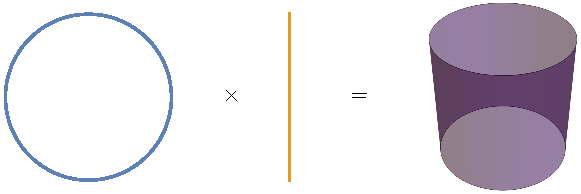
\includegraphics[width=.85\linewidth]{figures/circle-times-line-cylinder.pdf}\par}
\end{Example}

知道仿射簇的乘积本身也是仿射簇, 是研究乘积的重要第一步. 不过, 要研究坐标环, 维数和切空间, 还需要了解它们的消没理想.

\begin{Proposition}{乘积的消没理想}\leavevmode\label{prop:vanishing-ideal-of-product}
设 $X\subseteq\mathbb{A}^{m}$ 和 $Y\subseteq\mathbb{A}^{n}$ 为仿射簇. 则
\[
  \mathcal{I}(X\times Y)=\langle\mathcal{I}(X)\rangle+\langle\mathcal{I}(Y)\rangle,
\]
其中把 $\mathcal{I}(X)\subseteq K[x_{1},\ldots,x_{m}]$ 和 $\mathcal{I}(Y)\subseteq K[y_{1},\ldots,y_{n}]$ 看作较大多项式环 $K[x_{1},\ldots,x_{m},\allowbreak y_{1},\ldots,y_{n}]$ 的子集.
\end{Proposition}

\BookPairedNote
  {注意, 把 $\mathcal{I}(X)$ 和 $\mathcal{I}(Y)$ 看成 $K[x_{1},\ldots,x_{m},y_{1},\ldots,y_{n}]$ 的子集时, 它们不是理想. 所以先取它们各自生成的理想, 再取理想的和.}
  {回忆, 理想的和定义为 $I+J=\{a+b\mid a\in I,\ b\in J\}$.}
给定生成元 $\mathcal{I}(X)=\langle f_{1},\ldots,f_{k}\rangle$ 和 $\mathcal{I}(Y)=\langle g_{1},\ldots,g_{\ell}\rangle$, Proposition~\ref{prop:vanishing-ideal-of-product} 蕴含 (Exercise~\ref{ex:product-ideal-from-generators})
\[
  \mathcal{I}(X\times Y)=\langle f_{1},\ldots,f_{k},g_{1},\ldots,g_{\ell}\rangle
    \subseteq K[x_{1},\ldots,x_{m},y_{1},\ldots,y_{n}].
\]

\begin{Proof}\textbf{of Proposition~\ref{prop:vanishing-ideal-of-product}.}\quad
注意 $\langle\mathcal{I}(X)\rangle$ 的一般元素形如
\[
  h_{1}f_{1}+\cdots+h_{k}f_{k},
\]
其中 $h_{1},\ldots,h_{k}\in K[x_{1},\ldots,x_{m},y_{1},\ldots,y_{n}]$, 且 $f_{1},\ldots,f_{k}\in\mathcal{I}(X)$. 将任意这样的多项式在 $(a,b)\in X\times Y$ 处取值, 得
\[
  h_{1}(a,b)f_{1}(a)+\cdots+h_{k}(a,b)f_{k}(a)=0,
\]
因为对所有 $a\in X$, 有 $f_{1}(a)=\cdots=f_{k}(a)=0$. 类似的论证表明, $\langle\mathcal{I}(Y)\rangle$ 中的任意多项式在 $X\times Y$ 的每一点处都取值为零. 所以 $\langle\mathcal{I}(X)\rangle+\langle\mathcal{I}(Y)\rangle$ 的每个多项式都在 $X\times Y$ 上取值为零, 这表明
\[
  \langle\mathcal{I}(X)\rangle+\langle\mathcal{I}(Y)\rangle\subseteq\mathcal{I}(X\times Y).
\]

为证明反向包含, 设 $h\in\mathcal{I}(X\times Y)$. 总能找到形如
\begin{equation}\label{eq:polynomial-sum-of-separated-products}
  h=f_{1}g_{1}+\cdots+f_{k}g_{k}
\end{equation}
的表达式, 其中 $f_{1},\ldots,f_{k}\in K[x_{1},\ldots,x_{m}]$, 且 $g_{1},\ldots,g_{k}\in K[y_{1},\ldots,y_{n}]$ (例如, 将 $h$ 写成单项式之和, 再在每个单项式中把 $x$ 变量和 $y$ 变量分开). 对任意形如 \eqref{eq:polynomial-sum-of-separated-products} 的表达式, 重排后可设 $g_{1},\ldots,g_{j}\notin\mathcal{I}(Y)$, 而 $g_{j+1},\ldots,g_{k}\in\mathcal{I}(Y)$. 固定一个使 $j$ 最小的这种表达式. 对这个 $j$ 最小的表达式, 我们断言 $f_{1},\ldots,f_{j}\in\mathcal{I}(X)$, 由此得到
\[
  \begin{aligned}
    h&=f_{1}g_{1}+\cdots+f_{j}g_{j}+f_{j+1}g_{j+1}+\cdots+f_{k}g_{k}\\
     &\in\langle\mathcal{I}(X)\rangle+\langle\mathcal{I}(Y)\rangle,
  \end{aligned}
\]
从而结论得证.

为证明断言, 反设 $f_{1},\ldots,f_{j}$ 中有一个不属于 $\mathcal{I}(X)$. 不妨设对某个 $a\in X$ 有 $f_{1}(a)\neq0$. 定义
\[
  g=h(a,y)=f_{1}(a)g_{1}+f_{2}(a)g_{2}+\cdots+f_{k}(a)g_{k}
    \in K[y_{1},\ldots,y_{n}].
\]
由于 $h$ 在 $X\times Y$ 上取值为零, 可知 $g\in\mathcal{I}(Y)$. 解出 $g_{1}$ 得
\[
  g_{1}=f_{1}(a)^{-1}\bigl(g-f_{2}(a)g_{2}-\cdots-f_{k}(a)g_{k}\bigr).
\]
将该表达式代入 \eqref{eq:polynomial-sum-of-separated-products} 中的 $g_{1}$, 得到 $h$ 的一个如下形式的表达式:
\[
  \begin{aligned}
    h={}&\bigl(f_{2}-f_{1}(a)^{-1}f_{2}(a)f_{1}\bigr)g_{2}+\cdots\\
        &{}+\bigl(f_{k}-f_{1}(a)^{-1}f_{k}(a)f_{1}\bigr)g_{k}+f_{1}(a)^{-1}f_{1}g.
  \end{aligned}
\]
在这个新表达式中, $g_{2},\ldots,g_{j}\notin\mathcal{I}(Y)$, 而 $g_{j+1},\ldots,g_{k},g\in\mathcal{I}(Y)$, 与 $j$ 的最小性矛盾, 证明完毕.
\end{Proof}

Proposition~\ref{prop:vanishing-ideal-of-product} 使我们可以计算乘积的坐标环:
\[
  K[X\times Y]=\frac{K[x_{1},\ldots,x_{m},y_{1},\ldots,y_{n}]}
    {\langle\mathcal{I}(X)\rangle+\langle\mathcal{I}(Y)\rangle}.
\]
不过, 这个描述有一点令人不满意: 它要求从外在角度把 $X$ 和 $Y$ 都看作仿射空间的子集, 而不是只看作仿射簇的同构类. 因此自然会问: 能否仅用两个坐标环 $K[X]$ 和 $K[Y]$ 从内在角度计算坐标环 $K[X\times Y]$?

这个问题最理想的答案是给出一种代数运算 $\star$, 使得对所有仿射簇 $X$ 和 $Y$ 都有
\[
  K[X]\star K[Y]=K[X\times Y].
\]
无论 $\star$ 是什么, 它必有一个特例
\[
  K[x]\star K[y]=K[x,y],
\]
这是取 $X=Y=\mathbb{A}^{1}$, 从而 $X\times Y=\mathbb{A}^{2}$ 得到的.

这时读者或许会想, 目前知道哪些方法, 可以把两个 $K$-代数 $A$ 和 $B$ 合成一个新 $K$-代数 $A\star B$? 首先想到的运算可能是直和 $A\oplus B$. 可惜这并不是所需的运算. $A\oplus B$ 上的自然环结构是逐分量的:
\[
  \begin{aligned}
    (a_{1},b_{1})+(a_{2},b_{2})&=(a_{1}+a_{2},b_{1}+b_{2}),\\
    (a_{1},b_{1})\cdot(a_{2},b_{2})&=(a_{1}a_{2},b_{1}b_{2}),
  \end{aligned}
\]
读者可验证 (Exercise~\ref{ex:direct-sum-of-nonzero-rings-is-not-domain}), 这决不会产生整环. 所以 $K[x,y]$ 不可能与 $K[x]\oplus K[y]$ 相同.

我们很快会看到, 运算 $\star$ 的正确选择是 $K$-代数的张量积. 第~\ref{sec:tensor-products-of-modules} 和~\ref{sec:tensor-products-and-bilinearity}~节发展张量积的代数基础, 最后在第~\ref{sec:coordinate-rings-of-products}~节证明, 张量积确实给出了仿射簇乘积的坐标环. 不过, 在深入张量积之前, 先在第~\ref{sec:geometric-properties-of-products}~节研究乘积的关键几何性质, 回答关于不可约性, 维数和光滑性的自然问题.

\BookExerciseHeading
\begin{BookExercises}
  \item\label{ex:draw-product-finite-set-and-line} 令 $X=\mathcal{V}(x^{2}-1)\subseteq\mathbb{A}^{1}$ 和 $Y=\mathcal{V}(y-z)\subseteq\mathbb{A}^{2}$. 画出 $X\times Y\subseteq\mathbb{A}^{3}$ 在 $\mathbb{R}$ 上的图形.
  \item\label{ex:recognize-product-of-finite-sets} 画出仿射簇
  \[
    Z=\mathcal{V}(x+z^{2}-z,x)\subseteq\mathbb{A}^{3}=\mathbb{A}^{2}\times\mathbb{A}^{1}
  \]
  在 $\mathbb{R}$ 上的图形. 是否存在仿射簇 $X\subseteq\mathbb{A}^{2}$ 和 $Y\subseteq\mathbb{A}^{1}$ 使 $Z=X\times Y$? 若是, 给出这样的 $X$ 和 $Y$ 的一个例子. 若否, 如何看出?
  \item\label{ex:coordinate-planes-as-product-or-not} 画出仿射簇
  \[
    Z=\mathcal{V}(xyz)\subseteq\mathbb{A}^{3}=\mathbb{A}^{2}\times\mathbb{A}^{1}
  \]
  在 $\mathbb{R}$ 上的图形. 是否存在仿射簇 $X\subseteq\mathbb{A}^{2}$ 和 $Y\subseteq\mathbb{A}^{1}$ 使 $Z=X\times Y$? 若是, 给出这样的 $X$ 和 $Y$ 的一个例子. 若否, 如何看出?
  \item\label{ex:finite-product-of-affine-varieties} 将 Proposition~\ref{prop:product-of-affine-varieties-is-affine} 推广到有限个仿射簇的乘积, 并证明.
  \item\label{ex:product-ideal-from-generators} 设 $X\subseteq\mathbb{A}^{m}$ 和 $Y\subseteq\mathbb{A}^{n}$ 为仿射簇. 若 $\mathcal{I}(X)=\langle f_{1},\ldots,f_{k}\rangle$ 且 $\mathcal{I}(Y)=\langle g_{1},\ldots,g_{\ell}\rangle$, 证明
  \[
    \mathcal{I}(X\times Y)=\langle f_{1},\ldots,f_{k},g_{1},\ldots,g_{\ell}\rangle
      \subseteq K[x_{1},\ldots,x_{m},y_{1},\ldots,y_{n}].
  \]
  \item\label{ex:products-of-affine-varieties-are-intrinsic} 设 $X,X',Y,Y'$ 为仿射簇, 且 $X\cong X'$ 和 $Y\cong Y'$. 证明
  \[
    X\times Y\cong X'\times Y'.
  \]
  换句话说, 仿射簇的乘积是内在的.
  \item\label{ex:direct-sum-of-nonzero-rings-is-not-domain} 证明若 $A$ 和 $B$ 是非零环, 则配备逐分量加法和乘法的环 $A\oplus B$ 不是整环.
\end{BookExercises}
